Taisant sukurtą algoritmą buvo pastebėta, kad algoritmas turi trūkumą. Jei apskaičiuojamas tinklas yra sugrupuojamas į 2 grupes, iš kurių viena neveda link tikslo, tai ta grupė "išsiurbia srautą".

Pavyzdžiui, jeigu yra duotas tinklas $N=\{V=\{0, 1, 2, 3, 4\}, E=\{0 \rightarrow 1, 1 \rightarrow 2, 1 \rightarrow 4, 2 \rightarrow 3, 3 \rightarrow 2\}, u=\{(0 \rightarrow 1) = 10, (1 \rightarrow 2) = 5, (2 \rightarrow 3) = 5, (3 \rightarrow 2) = 10, (1 \rightarrow 4) = 10\}\}$, kurio šaltinis yra 0, o tikslas 4  \ref{fig:trukumas}.
\begin{figure}[h]
	\caption{Tinklo, kurio maksimalaus srauto algoritmas negali korektiškai apskaičiuoti, pavyzdys}
	\centering
	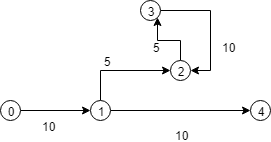
\includegraphics[width=0.5\textwidth]{img/trukumas.png}
	\label{fig:trukumas}
\end{figure}

Grupavimo funkcija sugrupuoja tinklą $N$ į grupes $G_1=\{V=\{0, 1, 4\}, E={0 \rightarrow 1, 1 \rightarrow 4, 1 \rightarrow m2}, u=\{(0 \rightarrow 1) = 10, (1 \rightarrow m2) = 5, (1 \rightarrow 4) = 10\}\}$ ir  $G_2=\{V=\{m2, 2, 3\}, E={m2 \rightarrow 2, 2 \rightarrow 3, 3 \rightarrow2}, u=\{(2 \rightarrow 3) = 5, (3 \rightarrow 2) = 10\}\}$, kur grupės $G_1$ šaltinis yra 0,  tikslai - m2 ir 4, o grupės $G_2$ šaltinis yra m2, tikslo grupė $G_2$ neturi  \ref{fig:trukumoGrupes}.
\begin{figure}[h]
	\caption{Tinklo, kurio maksimalaus srauto algoritmas negali korektiškai apskaičiuoti, pavyzdys}
	\centering
	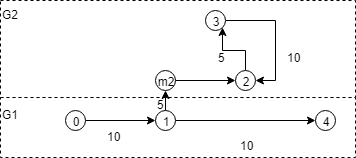
\includegraphics[width=0.5\textwidth]{img/trukumoGrupes.png}
	\label{fig:trukumoGrupes}
\end{figure}

Tada apskaičiuojant grupės $G_1$ maksimalius srautus bus gauti rezultatai: maksimalus srautas su tikslu m2 yra lygus 5, o su tikslu 4 - 5. Grupė $G_2$ neturi tikslo, tad su ja jokių skaičiavimų nevykdoma. Tad apskaičiuotas tinklo srautas yra 5, kai tikras tinklo N srautas yra 10. 